\documentclass[11pt]{article}

% Packages
\usepackage{amsmath, amsthm, amssymb}
\usepackage{hyperref}
\usepackage{graphicx}
\usepackage[utf8]{inputenc}
\usepackage{geometry}
\usepackage{xspace}
\usepackage[capitalize,noabbrev]{cleveref}

%\usepackage{minipage}
%\usepackage{mdframe}
\geometry{a4paper, margin=1in}
\usepackage{tikz}
\usetikzlibrary{shapes.geometric, arrows, positioning}

% Theorem Environments
\newtheorem{theorem}{Theorem}
\newtheorem{claim}{Claim}
\newtheorem{remark}{Remark}
\newtheorem{lemma}[theorem]{Lemma}
\newtheorem{corollary}[theorem]{Corollary}
\newtheorem{definition}[theorem]{Definition}
\newtheorem{proposition}[theorem]{Proposition}

\usepackage{enumitem}
\usepackage{mdframed}

\newcommand{\elaine}[1]{{\color{red} [elaine: #1]}}
\newcommand{\ignore}[1]{}
\newcommand{\sk}{\ensuremath{{\sf sk}}\xspace}
\newcommand{\DB}{\ensuremath{{\sf DB}}\xspace}

% Document Informatio n
\title{{\Large Cryptography meets algorithms (15893) Lecture Notes}\\[5pt]
{\bf Lecture 5: Piano: A Simple Preprocessing PIR Scheme}}
\author{Scribe: Tanisha Saxena}
\date{\today}

\begin{document}

\maketitle

% Please create a file named noteX.tex, where X is the number of the course. 
% Only edit the noteX.tex if possible.
% If you want to define macros, please have them inside the noteX.tex file.

{
\newcommand{\PRF}{\ensuremath{{\sf PRF}}}



%\section{PIANO: An Extremely Simple PIR}

\section{Motivation}
Recall that in previous lectures, we talked about classical PIR where the server stores the original database ($\mathsf{DB}$) unencoded and there's no preprocessing. Classical PIR requires the server to look through each element of the database, otherwise the server can deduce that the skipped elements are unimportant to the client. Beimel et.~al~\cite{beimel2000reducing} proved that a server in classical PIR must have linear computation per query.
Linear computation will unlikely 
scale for many real-world applications, e.g., private DNS and private 
web search. 
To avoid this linear computation barrier,  
more recent PIR schemes 
considered 
the preprocessing model~\cite{beimel2000reducing,sublinearpir}. 
%\elaine{cite also corrigan-gibbs and kogan}
In this lecture, we will show how we can achieve sublinear computation
per query in the preprocessing model. 
%, with respect to the database. 
%Following this discovery, 
%Beimel et. al proved that preprocessing can overcome this complexity barrier. In this lecture, we'll understand how they did that.

\section{Background}
%As we learned from guest lecturer Wei-Kai Lin, 
Previous works have considered 
main models of pre-processing: 

%\begin{definition}[Types of Preprocessing in PIR]
%    \hfill
    \begin{itemize}
        \item \textbf{Public preprocessing:} The server computes an encoding of the dabase 
$\mathsf{DB}$. This preprocessing is shared
globally by all clients. %globally and maintains the same encoding scheme for all clients.
        \item \textbf{Client-specific preprocessing:} 
The server performs a preprocessing protocol with each client. The client is stateful, i.e., each client maintains some local state called the \textbf{hint}.
    \end{itemize}
%\end{definition}
%For this lecture, we'll be using client-specific preprocessing to achieve faster than linear time complexity.

The ``doubly-efficient PIR'' 
scheme Wei-Kai talked about in his guest lecture 
is in the public preprocessing model.
In this lecture, 
we will describe a scheme called Piano by Zhou et al.~\cite{zhou2023piano} 
that uses the client-specific preprocessing model.


%\section{Goals}
Piano achieves $O(\sqrt{n})$ server time and $O(\sqrt{n})$ bandwidth per query, 
assuming $\widetilde{O}(\sqrt{n})$ client space. 
%The scheme assumes that pseudorandom functions (PRF) exists (One-way Function).
The only cryptographic primitive Piano relies is pseudorandom functions (PRFs).


\section{Warmup Scheme: Supporting A Single Query}
As a warmup, we will show a scheme that supports only one query after the preprocessing. 
\ignore{
As a warmup, we will first make some simplifying assumptions: we will
assume that there are only $\sqrt{n}$ queries after 
the preprocessing 
phase, and all queries for {\it random and distinct} indices.
We will describe how to extend this scheme to support
unbounded and arbitrary queries later.
}
%assume each query is random (i.e. the index of each message the client wants is randomly chosen), and that there are up to $\sqrt{n}$ unique queries. Basically, we're assuming our current queries are bounded and random. We'll remove this restriction later and are only using it now for the sake of ease.


Given a database $\mathsf{DB}$, we split the $n$ indices 
into $\sqrt{n}$ chunks of size $\sqrt{n}$.
We assume $n$ is a perfect square.

\begin{center}
    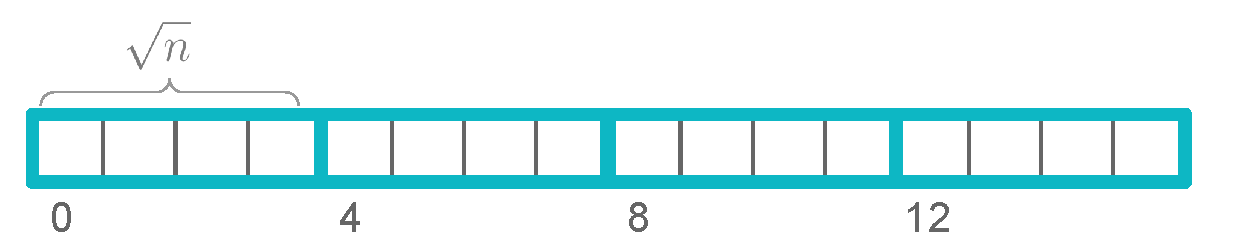
\includegraphics[scale=0.6]{chunks}\\
{\bf Figure:} The database indices are divided into $\sqrt{n}$ chunks of size $\sqrt{n}$. 
\end{center}

\paragraph{Random set.}
We will sample a random set 
of size $\sqrt{n}$ by sampling one random index from
each of the $\sqrt{n}$ chunks, as illustrated in the picture below. 


\begin{center}
    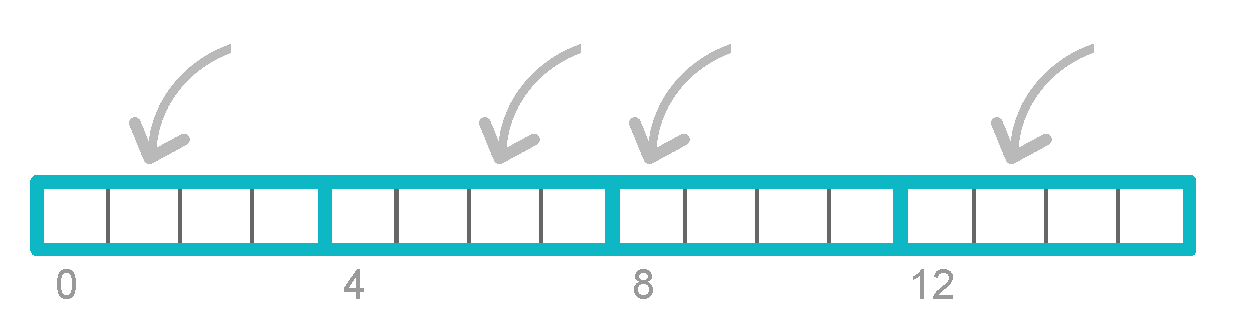
\includegraphics[scale=0.6]{piano-sample}\\
{\bf Figure:} We sample a random set of size $\sqrt{n}$ by sampling one random index per chunk.
\end{center}

Given a random set $S$ sampled according to the above procedure,
we define the notation
\[
{\sf Parity}(S) = \oplus_{i \in S}{\sf DB}[i] 
\] 


\paragraph{Describing a set with a single PRF key.}
We need a succinct way to represent each set sampled as above.
We can represent each 
set using a PRF key $\sk$.
Supposewe have a 
pseudorandom function family 
$\PRF:\{0,1\}^\lambda\times \{0,\dots,\sqrt{n}-1\}\to \{0,\dots,\sqrt{n}-1\}$. 
%associated some key $k$.
%We can use this PRF to construct a random set.
Given a PRF key $\sk \in \{0, 1\}^\lambda$, 
we can compute a pseudorandom 
index from each chunk as follows:
the index from the 
the $i$-th chunk is $\PRF_\sk(i)+i\cdot\sqrt{n}$ where $i \in \{0, \ldots, \sqrt{n}-1\}$. 
In other words,
$\PRF_\sk(i)$ outputs the offset within the 
$i$-th chunk.

%So each set only takes $\lambda$-bit to describe, 
%and the client space is $O_\lambda(\sqrt{n}\log n)$.
%

Henceforth, we use the notation ${\sf Set}(\sk)$ to denote
the pseudorandom set generated by the PRF key $\sk \in \{0, 1\}^\lambda$.
Given an index $j \in \{0,\dots,\sqrt{n}-1\}$,
we can determine if 
$j \in {\sf Set}(\sk)$ in $O_\lambda(1)$ time, 
by checking 
if $\PRF_\sk(i) + i \sqrt{n} = j$ where $i = {\sf chunk}(j)$ denotes
the chunk that index $j$ belongs to.



\paragraph{Preprocessing.}
The client wants to prepare and store the following information during the preprocessing:  
\begin{itemize}
\item 
{\bf Hint table.}
First, the client samples
$L = \widetilde{O}(\sqrt{n})$
pseudorandom sets\footnote{We use $\widetilde{O}(\cdot)$ to hide
a superlogarithmic factor.} represented by PRF keys $\sk_1, \ldots, \sk_L$.
%random sets $S_1, \ldots, S_L$.
Further, for each $i \in [L]$, the client will 
find out the parity 
$p_i = {\sf Parity}({\sf Set}(\sk_i))$, and store the parity bit alongside $\sk_i$.
The resulting table $\{(\sk_i, p_i)\}_{i \in [L]}$ 
stored by the client
is called the hint table.
Each entry $(\sk_i, p_i)$ in the hint table is called a hint.
\item 
{\bf Replacement entries.}
For each chunk $i \in \{0, \ldots, \sqrt{n}-1\}$, the client
samples $\widetilde{O}(1)$
random indices within the chunk; moreover, for each index $r$ sampled,
it wants to learn ${\sf DB}[r]$.  
As a result, the client will store $\widetilde{O}(1)$
replacement entries of the form $(r, \DB[r])$ for each chunk. 
\end{itemize}

It takes $\widetilde{O}_\lambda(\sqrt{n})$ space to
store the hint table and the replacement entries.

\begin{claim}
The client can find out all $L$ parities
as well as
the database at the sampled indices (for the replacement entries)
by making a streaming pass over the database, consuming
only $\widetilde{O}_\lambda(\sqrt{n})$ space.
\end{claim}
How to accomplish the above with a single streaming pass is left as an exercise.

\paragraph{Making a query.}
%A client makes queries in the following way. 
%Consider a client that wants to query on index $i = 6$. 
Suppose the client wants to read index
$q \in \{0, 1, \ldots, n-1\}$.
It will do the following: 
\begin{itemize}
\item 
Find a hint $(\sk^*, p^*)$
from its hint table such that $q \in {\sf Set}(\sk^*)$.
\item 
Let $i = {\sf chunk}(q)$, obtain the next unconsumed
replacement entry belonging to the $i$-th chunk, denoted $(r, \DB[r])$,
where index $r$ belongs
to the $i$-th chunk.
\item 
Let $S = {\sf Set}(\sk^*)$ but 
replace the query $q$ with $r$. 
Send $S$ to the server. 
\item 
Wait for the server to return 
$p = {\sf parity}(S)$.
Reconstruct the answer $p \oplus p^* \oplus \DB[r]$ where the client knows $\DB[r]$
from the replacement entry consumed.
\end{itemize}

Checking correctness of the answer is easy and left as an exercise.

\paragraph{Security of one query.}
Observe that the set $S$ sent to the server is indisitinguishable
from a randomly sampled set (i.e., sampling one random index per chunk).  
In particular, the client first searches for a set subject to containing the query $q$.
If the PRF were a random function, then this set would have the same distribution as
``sampling a random set subject to 
containing $q$''.
When we replace $q$ with 
%Then, it replaces $q$ with 
a random index from the same chunk, the resulting set
would have the same distribution as a randomly sampled set.

\section{Next Step: Supporting a Bounded Number of Random, Distinct Queries}
The scheme so far can support one query, but 
an issue arises if the client continues to make more queries.

The question is, 
once we make a query, 
what happens to the hint that is consumed? 
If we keep the hint, then the next time the same hint
is consumed, e.g., due to a different query, the server  
can learn the query index $q$ that was scooped out earlier.  
If we simply remove the hint, it skews the distribution of the sets 
in the hint table.
Specifically, the remaining sets have slightly lower
probability of containing the query $q$. 
This will also cause slight information leakage 
in future queries.

To avoid information leakage over multiple queries, 
the idea is the following. 
Imagine that the PRF were a random function.
Recall that the consumed set has the same distribution
as ``a randomly sampled set subject to containing the query $q$''.
When it is consumed, 
we want to replace it with a freshly sampled
set subject to containing $q$ --- of course, we will also need to know the parity
of this new set to maintain the correctness of the scheme. 

To achieve this, the client will also prepare  
some backup sets as mentioned below.

\paragraph{Backup sets.}
During preprocessing, 
for each chunk, the client will prepare 
$\widetilde{O}(1)$ number of backup sets.
A backup
set for a chunk $i \in \{0, \ldots, \sqrt{n}-1\}$ 
is sampled as follows:
sample one random index 
for every chunk $j \neq i$.
One can imagine that 
a backup set a random set except for leaving a hole in chunk $i$.
Each backup set (for some chunk $i$) 
can also be described with a PRF key $\sk$, except that 
we will never have to evaluate $\PRF_{\sk}(i)$.

\newpage
\begin{center}
    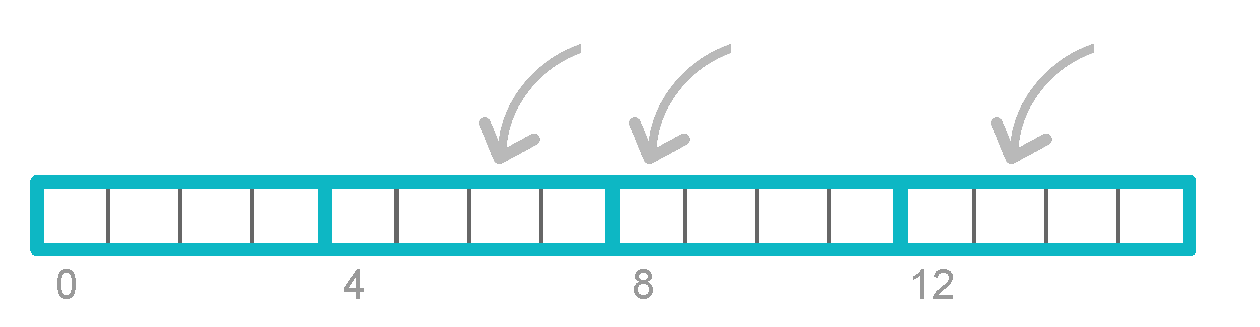
\includegraphics[scale=0.6]{piano-backupset}\\
{\bf Figure:} %The database indices are divided into $\sqrt{n}$ chunks of size $\sqrt{n}$. 
A backup set for chunk $0$ contains a random index per chunk except for chunk $0$. 
\end{center}



The client also wants to learn and store the parities of all backup sets
during preprocessing.
This can be accomplished in the same streaming pass 
mentioned above.


\paragraph{Refreshing a consumed hint.}
During a query for index $q$, 
suppose the client consumes some hint. %$(\sk^*, p^*)$. 
It will fetch
the next unconsumed backup set 
for chunk $i = {\sf chunk}(q)$.
along with its parity denoted $(\sk', p')$.
It will replace the consumed hint with $(\sk' \cup \{q\}, p' \oplus \DB[q])$,
where $\sk' \cup \{q\}$ is used to mean ``fill in the hole in the backup set represented
by $\sk'$ with $q$''; further, 
$p' \oplus \DB[q]$ is the correct parity of the set when we fill in the hole with $q$.
The client knows $\DB[q]$ because it has just reconstructed the answer to the present query.

Note that now in this scheme, 
each hint can be of the form $(\sk, p)$, or $(\sk \cup \{q\}, p)$, depending on whether
it has been refreshed or not.


\paragraph{Why bounded, random and distinct
queries.}
The scheme so far will work as long as we do not exhaust
the replacement entries and the backup sets.

Suppose there are at most $\sqrt{n}$ queries after the proprocessing,
and moreover, all queries are random and distinct.
We can think of the $\sqrt{n}$ chunks
as $\sqrt{n}$ bins, and 
each query will land in a random bin.
By Chernoff bound,  
except with negligible probability, 
no bin will receive more than super-logarithmically many queries.
This is why we provisioned $\widetilde{O}(1)$ queries (i.e., superlogarithmically many)
per chunk during preprocessing. 

\section{Supporting Unbounded and Arbitrary Queries}
 
\section{TO Edit}


\ignore{
Suppose the index we want to query is stored in some set $S_2 = (0, 6, 9, 5)$ -- note that this set can be found amongst the $\sqrt{n}$ sets with non-negligible probability. To query on this, we simply sample some random $r$ and send $S^* = (0, r, 9, 5)$ to the server. In return, we get $\mathsf{Parity}(S^*)$. With the help of our hint, we can compute $\mathsf{Parity}(S_2) \oplus \mathsf{Parity}(S^*) \oplus \mathsf{DB}[r] = \mathsf{DB}[i]$.
}




%\paragraph{Describing a pseudorandom set with a single PRF key.}

\ignore{
\begin{definition}[]
    \hfill \\
    \textbf{Parity:} Given a set of indices $S = \{i_1, i_2, \dots, i_{\sqrt{n}}\}$, we define $\mathsf{Parity}(S)$ as \hfill \\ $\mathsf{DB}(i_1) \oplus \mathsf{DB}(i_2) \oplus \dots \oplus \mathsf{DB}(i_{\sqrt{n}})$
\end{definition}
}




\ignore{In the preprocessing phase,
the client will randomly sample roughly $\Theta(\sqrt{n}\log n)$ random sets.
For each set, it samples one random index in each chunk.
The cilent will then preprocess all the  parities for those sets.
The preprocessing is done by streamingly download the whole database and dynamically update all the parities.
}


\paragraph{Compressing client hints with PRFs.}
Naively, to store all the hints, it takes $\Omega(n\log n)$ space.
Assume we have a $\PRF:\{0,1\}^\lambda\times \{0,\dots,\sqrt{n}-1\}\to \{0,\dots,\sqrt{n}-1\}$, associated some key $k$.
We can use this PRF to construct a random set.
We define the element in the $i$-th chunk to be $\PRF_k(i)+i\cdot\sqrt{n}$.
So each set only takes $\lambda$-bit to describe, and the client space is $O_\lambda(\sqrt{n}\log n)$.
%We can prove the correctness of this method with the following intuition: given some $i \in [n]$, $i$ is the index of an element within one of the $\sqrt{n}$ sets of $S$. Thus, we can get the $chunk \text{ } id$ of $i$ simply by determining which chunk it's in, and then we call the PRF on that id to get the offset, all of which is within our complexity bounds.

\paragraph{Making Queries.}
A client makes queries in the following way. Consider a client that wants to query on index $i = 6$. Suppose the index we want to query is stored in some set $S_2 = (0, 6, 9, 5)$ -- note that this set can be found amongst the $\sqrt{n}$ sets with non-negligible probability. To query on this, we simply sample some random $r$ and send $S^* = (0, r, 9, 5)$ to the server. In return, we get $\mathsf{Parity}(S^*)$. With the help of our hint, we can compute $\mathsf{Parity}(S_2) \oplus \mathsf{Parity}(S^*) \oplus \mathsf{DB}[r] = \mathsf{DB}[i]$.

However, this raises a new issue. Suppose the new index we want to query is also in $S_2$. Then if we were to send an $S^{**}$ with a different value replaced with $r$, the server would be able to recognize that $S^{**}$ is similar to $S^*$ and would then deduce some information about $i$. We also can't just delete $S_2$ to avoid this issue, because this would skew the distribution of the sets and would still give the server information about the query. The solution is that we use ``backup" sets to replace the ones we've already used.

\paragraph{Backup Sets}
Alongside the hint, each client will store a polylog number of ``backup" sets for each of the $\sqrt{n}\log n$ sets. Each backup set for chunk $j$ is stored assuming the $j$th index is missing, and the client simply stores the parity of the backup set. Examples include: $\mathsf{Parity}(0, \_\_, 9, 5)$ and $\mathsf{Parity}(0, \_\_, 8, 13)$ for the second chunk. 

\paragraph{Removing the ``Bounded" and ``Random" Queries Assumptions}
Note that within each set of $\sqrt{n}$ queries, the client can cache the results of the last $\sqrt{n}$ queries. Whenever it has a repeated query, it can make a dummy query and find the cached result. When we do the queries for the first $\sqrt{n}$ queries, we can simultaneously do the preprocessing to prepare for the next $\sqrt{n}$ queries.

\begin{center}
    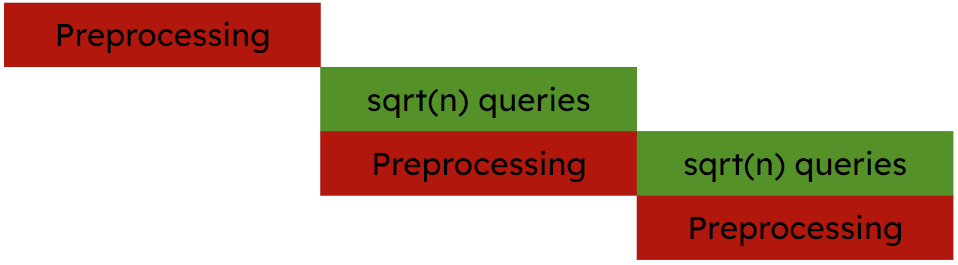
\includegraphics[scale=0.77]{scrbimg.png}
\end{center}

And as easily as that, we have removed the bounded and random queries restrictions!

\paragraph{Applications}
This scheme is much faster than non-processing PIR schemes. Because of that, it has many applications for fast secrecy. For example, \href{https://haveibeenpwned.com/}{haveibeenpwned.com}, a website that checks if a user's password has been in a data breach, would be able to more efficiently run a search on a user's password without actually ever knowing what the password is.

}
\bibliographystyle{alpha}
\bibliography{refs.bib}
\end{document}
